\chapter*{Proposition 32}



\begin{figure*}[ht]
    \begin{center}
    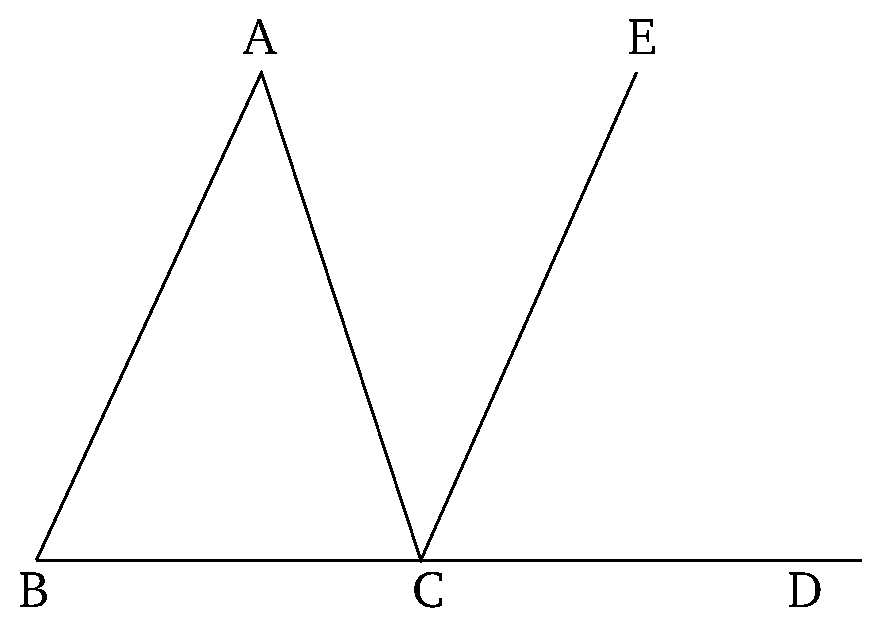
\includegraphics[width=0.5\linewidth]{figures/fig32e.eps}
    \label{fig:prop_32}
    \end{center}
\end{figure*}

In any triangle,  (if) one of the sides (is) produced  (then) the external
angle is equal to the (sum of the) two internal and opposite (angles), and the (sum of the) three
internal angles of the triangle is equal to two right-angles.

Let $ABC$ be a triangle, and let one of its sides $BC$ have been produced to $D$.
I say that the external angle $ACD$ is equal to the (sum of the) two internal and opposite
angles $CAB$ and $ABC$, and the (sum of the) three internal angles of the triangle---$ABC$, $BCA$, and $CAB$---is equal to two right-angles.

For let $CE$ have been drawn through point $C$ parallel to the straight-line
$AB$ [Prop.~1.31].

And since $AB$ is parallel to $CE$, and $AC$ has fallen across them, the alternate
angles $BAC$ and $ACE$ are equal to one another [Prop.~1.29]. Again,
since $AB$ is parallel to $CE$, and the straight-line $BD$ has fallen across them, 
the external angle $ECD$ is equal to the internal and opposite (angle)
$ABC$ [Prop.~1.29]. But $ACE$ was also shown (to be) equal to $BAC$. Thus, the whole
angle $ACD$ is equal to the (sum of the) two internal and opposite (angles) $BAC$ and $ABC$.

Let $ACB$ have been added to both. Thus, (the sum of) $ACD$ and $ACB$ is equal to
the (sum of the) three (angles) $ABC$, $BCA$, and $CAB$. But, (the sum of) $ACD$ and $ACB$ is equal
to two right-angles [Prop.~1.13]. Thus, (the sum of) $ACB$, $CBA$, and $CAB$ is also
equal to two right-angles.

Thus, in any triangle,  (if) one of the sides  (is) produced (then) the external
angle is equal to the (sum of the) two internal and opposite (angles), and the (sum of the) three
internal angles of the triangle is equal to two right-angles. (Which is)
the very thing it was required to show.


\section*{Commentary}

\begin{proposition}\label{proposition_32}\lean{Elements.Book1.proposition_32}\leanok
    If
\end{proposition}
\begin{proof}
    \uses{proposition_13,proposition_29,proposition_31}\leanok
\end{proof}
